% ITP 2026 Short Paper - PokemonLean
% Lightweight double-blind: anonymous option enabled
\documentclass[a4paper,UKenglish,cleveref,autoref,anonymous]{lipics-v2021}

\pdfoutput=1

% TikZ for figures
\usepackage{tikz}
\usetikzlibrary{shapes,arrows,positioning,fit,backgrounds,calc}

\bibliographystyle{plainurl}

\title{Formalizing Pok\'emon TCG in Lean 4: Semantics, Invariants, and a Certified Solver}

\subtitle{Short Paper}

\titlerunning{Formalizing Pok\'emon TCG in Lean 4}

% Authors are anonymized for double-blind review
\author{Anonymous Author(s)}{Anonymous Institution, Country}{anonymous@example.org}{}{}

\authorrunning{Anonymous}

\Copyright{Anonymous Author(s)}

\ccsdesc[500]{Software and its engineering~Formal software verification}
\ccsdesc[300]{Theory of computation~Program verification}
\ccsdesc[100]{Applied computing~Computer games}

\keywords{Formal verification, Lean 4, Game semantics, Trading card games, Certified algorithms}

\category{} 

\relatedversion{} 
%\relatedversiondetails{Full Version}{https://arxiv.org/abs/XXXX.XXXXX}

\supplementdetails{Software}{https://anonymous.4open.science/r/AnonymousLeanPokemon-8E76}

%\funding{}

%\acknowledgements{}

\begin{document}

\maketitle

\begin{abstract}
We present a formal model of the Pok\'emon Trading Card Game (TCG) in Lean~4, comprising small-step operational semantics, legality predicates, and global invariants verified across all reachable game states.
Our formalization includes 14 action types modeling core gameplay mechanics: playing cards, attaching energy, attacking, retreating, and turn management.
We prove key meta-theoretic properties including card conservation, bench limits, prize bounds, and the impossibility of winning on the first turn from a standard starting position.
As a payoff, we implement a \emph{certified solver} that selects the damage-maximal legal attack, with machine-checked proofs of both soundness (the returned attack is legal) and optimality (no legal attack deals more damage).
The formalization totals approximately 3{,}500 lines of Lean~4 code with over 80 proven theorems, demonstrating that proof assistants can tractably model the complex rule systems found in commercial trading card games.
\end{abstract}

%%%%%%%%%%%%%%%%%%%%%%%%%%%%%%%%%%%%%%%%%%%%%%%%%%%%%%%%%%%%%%%%%%%%%%%%%%%%%%%
\section{Introduction}
\label{sec:intro}
%%%%%%%%%%%%%%%%%%%%%%%%%%%%%%%%%%%%%%%%%%%%%%%%%%%%%%%%%%%%%%%%%%%%%%%%%%%%%%%

Trading card games (TCGs) present an interesting challenge for formal methods: they combine discrete state spaces with complex, interacting rule systems that evolve through expansions and errata.
The Pok\'emon TCG, with over 25 years of continuous development and thousands of unique cards, exemplifies this complexity.
Players must navigate energy attachment rules, type-based weakness and resistance modifiers, status conditions, evolution chains, and per-turn action limits---all while making strategically optimal decisions.

We present \textsc{PokemonLean}, a formalization of core Pok\'emon TCG mechanics in Lean~4~\cite{lean4,DBLP:conf/cav/MouraKADR15}.
Our contributions are:
\begin{enumerate}
\item A \textbf{small-step operational semantics} with 14 action types and decidable legality predicates (\cref{sec:semantics}).
\item \textbf{Global invariants} (``meta-safety'') proven to hold for all reachable game states, including card conservation, zone bounds, and the impossibility of first-turn victories (\cref{sec:invariants}).
\item A \textbf{certified solver} with machine-checked soundness and optimality theorems for attack selection (\cref{sec:solver}).
\end{enumerate}

\paragraph{Scope.}
Our model covers the core TCG rules: energy types, attacks with energy costs, weakness ($\times 2$) and resistance ($-30$), status conditions, evolution, retreat, trainer cards (items, supporters, tools), and prize mechanics.
We model a representative fragment sufficient to prove interesting properties while remaining tractable.
Excluded are: stadium cards with global effects, multi-prize EX/V/VMAX knockouts, and complex ability interactions beyond heal/draw effects.

%%%%%%%%%%%%%%%%%%%%%%%%%%%%%%%%%%%%%%%%%%%%%%%%%%%%%%%%%%%%%%%%%%%%%%%%%%%%%%%
\section{Game Model and Semantics}
\label{sec:semantics}
%%%%%%%%%%%%%%%%%%%%%%%%%%%%%%%%%%%%%%%%%%%%%%%%%%%%%%%%%%%%%%%%%%%%%%%%%%%%%%%

\paragraph{State Representation.}
A game state comprises two player states and an active player indicator (\cref{fig:gamestate}).
Each player state tracks: a deck, hand, bench (up to 5 Pok\'emon), active Pok\'emon (optional), discard pile, and prize cards.
A Pok\'emon in play carries its base card, accumulated damage, status condition, and attached energy.

\begin{figure}[t]
\centering
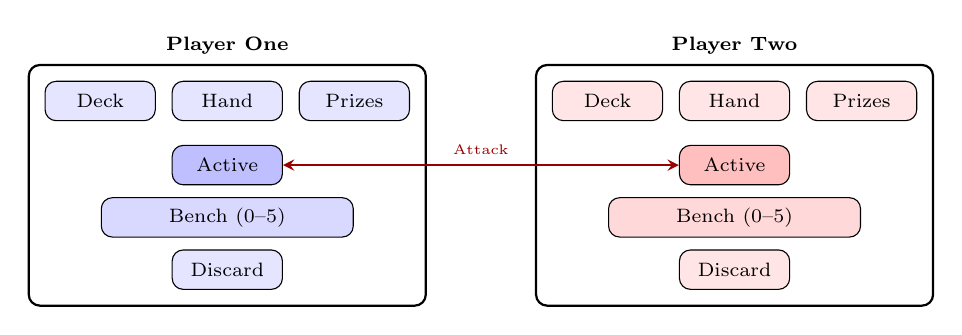
\begin{tikzpicture}[
    node distance=0.2cm,
    zone/.style={draw, rounded corners, minimum width=1.4cm, minimum height=0.5cm, font=\scriptsize},
    player/.style={draw, rounded corners, thick, inner sep=0.2cm},
    >=stealth
]
% Player One
\node[zone, fill=blue!10] (deck1) {Deck};
\node[zone, fill=blue!10, right=of deck1] (hand1) {Hand};
\node[zone, fill=blue!10, right=of hand1] (prizes1) {Prizes};
\node[zone, fill=blue!25, below=0.3cm of hand1] (active1) {Active};
\node[zone, fill=blue!15, below=0.15cm of active1, minimum width=3.2cm] (bench1) {Bench (0--5)};
\node[zone, fill=blue!10, below=0.15cm of bench1] (discard1) {Discard};
\node[player, fit=(deck1)(hand1)(prizes1)(active1)(bench1)(discard1), label=above:{\scriptsize\textbf{Player One}}] (p1) {};

% Player Two
\node[zone, fill=red!10, right=1.8cm of prizes1] (deck2) {Deck};
\node[zone, fill=red!10, right=of deck2] (hand2) {Hand};
\node[zone, fill=red!10, right=of hand2] (prizes2) {Prizes};
\node[zone, fill=red!25, below=0.3cm of hand2] (active2) {Active};
\node[zone, fill=red!15, below=0.15cm of active2, minimum width=3.2cm] (bench2) {Bench (0--5)};
\node[zone, fill=red!10, below=0.15cm of bench2] (discard2) {Discard};
\node[player, fit=(deck2)(hand2)(prizes2)(active2)(bench2)(discard2), label=above:{\scriptsize\textbf{Player Two}}] (p2) {};

% Battle arrow
\draw[<->, thick, red!60!black] (active1.east) -- node[above, font=\tiny] {Attack} (active2.west);
\end{tikzpicture}
\caption{Game state structure. Each player maintains six zones; active Pok\'emon battle each other.}
\label{fig:gamestate}
\end{figure}

\begin{figure}[t]
\begin{lstlisting}[basicstyle=\ttfamily\small,columns=flexible]
structure PokemonInPlay where
  card   : Card
  damage : Nat
  status : Option StatusCondition
  energy : List EnergyType

structure PlayerState where
  deck, hand, discard, prizes : List Card
  bench  : List PokemonInPlay
  active : Option PokemonInPlay
\end{lstlisting}
\caption{Core Lean types for game state representation.}
\label{fig:state}
\end{figure}

\paragraph{Actions and Step Function.}
We define an \texttt{Action} type with 14 constructors covering all major gameplay actions, following the structural operational semantics tradition~\cite{Plotkin2004} and the official Pok\'emon TCG rulebook~\cite{pokemon-tcg-rules}:

\begin{lstlisting}[basicstyle=\ttfamily\small,columns=flexible]
inductive Action
  | playPokemonToBench (card : Card)
  | playItem (card : Card)
  | playSupporter (card : Card)
  | attachEnergy (energyType : EnergyType)
  | attack (attackIndex : Nat)
  | retreat | endTurn | drawCard | ...
\end{lstlisting}

The transition function \texttt{step} implements the game rules, with type:
\[
\texttt{step : GameState} \to \texttt{Action} \to \texttt{Except StepError GameState}
\]
For example, playing a Pok\'emon to the bench requires the card to be in hand and the bench to have fewer than 5 Pok\'emon:

\begin{lstlisting}[basicstyle=\ttfamily\small,columns=flexible]
| .playPokemonToBench card =>
  match removeFirst card playerState.hand with
  | none => .error .cardNotInHand
  | some newHand =>
    if bench.length < benchLimit then
      .ok (addToBench card newHand)
    else .error .benchFull
\end{lstlisting}

\paragraph{Legality Predicates.}
For each action, we define a decidable legality predicate \texttt{Legal : GameState $\to$ Action $\to$ Prop}.
A key theorem establishes the correspondence between \texttt{Legal} and successful stepping:

\begin{theorem}[\texttt{step\_total\_for\_legal}]
For any state $s$ and action $a$, if $\mathit{Legal}(s, a)$ holds, then $\mathit{step}(s, a) = \mathit{ok}(s')$ for some $s'$.
\end{theorem}

The converse also holds: \texttt{step\_error\_iff\_not\_legal} establishes that stepping errors precisely when the action is illegal.

\paragraph{Damage Calculation.}
The damage pipeline applies weakness and resistance (\cref{fig:damage}):
$$\mathit{damage} = \max(0, (\mathit{base} + \mathit{effects}) \times \mathit{weakness} - \mathit{resistance})$$
where weakness doubles damage if the attacker's type matches the defender's weakness, and resistance subtracts 30.
We prove bounds on this calculation:

\begin{figure}[t]
\centering
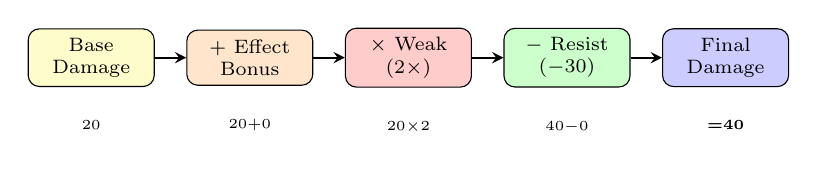
\begin{tikzpicture}[
    node distance=0.4cm,
    block/.style={draw, rounded corners, minimum width=1.6cm, minimum height=0.7cm, align=center, font=\scriptsize},
    arrow/.style={->, thick, >=stealth}
]
\node[block, fill=yellow!20] (base) {Base\\Damage};
\node[block, fill=orange!20, right=of base] (effects) {+ Effect\\Bonus};
\node[block, fill=red!20, right=of effects] (weak) {$\times$ Weak\\(2$\times$)};
\node[block, fill=green!20, right=of weak] (resist) {$-$ Resist\\($-$30)};
\node[block, fill=blue!20, right=of resist] (final) {Final\\Damage};
\draw[arrow] (base) -- (effects);
\draw[arrow] (effects) -- (weak);
\draw[arrow] (weak) -- (resist);
\draw[arrow] (resist) -- (final);
\node[below=0.3cm of base, font=\tiny] {20};
\node[below=0.3cm of effects, font=\tiny] {20+0};
\node[below=0.3cm of weak, font=\tiny] {20$\times$2};
\node[below=0.3cm of resist, font=\tiny] {40$-$0};
\node[below=0.3cm of final, font=\tiny\bfseries] {=40};
\end{tikzpicture}
\caption{Damage pipeline: Squirtle (Water) attacking Charmander (weak to Water).}
\label{fig:damage}
\end{figure}

\begin{theorem}[\texttt{damage\_nonneg}, \texttt{damageBounds}]
Damage is always $\geq 0$, and for any attack with base damage $b$ and defender with resistance $r$: $0 \leq \mathit{damage} \leq 2 \cdot (b + \mathit{bonus})$.
\end{theorem}

%%%%%%%%%%%%%%%%%%%%%%%%%%%%%%%%%%%%%%%%%%%%%%%%%%%%%%%%%%%%%%%%%%%%%%%%%%%%%%%
\section{Meta-Safety Invariants}
\label{sec:invariants}
%%%%%%%%%%%%%%%%%%%%%%%%%%%%%%%%%%%%%%%%%%%%%%%%%%%%%%%%%%%%%%%%%%%%%%%%%%%%%%%

We define reachability inductively from an initial game state:

\begin{lstlisting}[basicstyle=\ttfamily\small,columns=flexible]
inductive ReachableFrom (start : GameState) : GameState -> Prop
  | initial : ReachableFrom start start
  | step (h : ReachableFrom start s) (hLegal : Legal s a)
         (hStep : step s a = .ok s') : ReachableFrom start s'
\end{lstlisting}

\noindent We prove several invariants hold for all reachable states:

\begin{theorem}[\texttt{reachable\_card\_conservation}]
The total number of cards across all zones (deck, hand, bench, active, discard, prizes) is invariant: for any reachable state $s$, $\mathit{totalCardCount}(s) = \mathit{totalCardCount}(\mathit{initial})$.
\end{theorem}

\begin{theorem}[\texttt{reachable\_bench\_bounds}]
For any reachable state, both players' benches have at most 5 Pok\'emon: $|s.\mathit{playerOne}.\mathit{bench}| \leq 5 \land |s.\mathit{playerTwo}.\mathit{bench}| \leq 5$.
\end{theorem}

\begin{theorem}[\texttt{reachable\_prizes\_bounds}]
Prize counts remain in $[0, 6]$: $|s.\mathit{prizes}| \leq 6$ for both players in any reachable state.
\end{theorem}

\paragraph{No Turn-One Win.}
A particularly interesting invariant concerns the impossibility of winning on the first turn from a standard starting position.
We define \texttt{TurnOneActions} as the set of action sequences available on turn one (no attacking, since the going-first player cannot attack on turn one in standard rules):

\begin{theorem}[\texttt{no\_turn\_one\_win}]
For any sequence of actions $\vec{a}$ satisfying \texttt{TurnOneActions}, if $\mathit{stepMany}(\mathit{initial}, \vec{a}) = \mathit{ok}(s')$, then $\neg\mathit{hasWon}(\mathit{playerOne}, s')$.
\end{theorem}

This theorem captures a fundamental balance property of the game rules.

%%%%%%%%%%%%%%%%%%%%%%%%%%%%%%%%%%%%%%%%%%%%%%%%%%%%%%%%%%%%%%%%%%%%%%%%%%%%%%%
\section{Certified Attack Solver}
\label{sec:solver}
%%%%%%%%%%%%%%%%%%%%%%%%%%%%%%%%%%%%%%%%%%%%%%%%%%%%%%%%%%%%%%%%%%%%%%%%%%%%%%%

As a practical payoff, we implement a solver that selects the damage-maximal legal attack.
The core function \texttt{bestAttack} iterates through available attacks, filtering by energy cost legality and selecting the highest-damage option:

\begin{lstlisting}[basicstyle=\ttfamily\small,columns=flexible]
def bestAttack (attacker defender : PokemonInPlay) 
    : Option (Nat * Attack) :=
  bestAttackFrom attacker defender attacker.card.attacks
\end{lstlisting}

\noindent We prove two key properties:

\begin{theorem}[\texttt{bestAttack\_sound}]
If $\mathit{bestAttack}(a, d) = \mathit{some}(i, \mathit{atk})$, then $i < |a.\mathit{attacks}|$ and the energy cost of $\mathit{atk}$ is satisfied by $a.\mathit{energy}$.
\end{theorem}

\begin{theorem}[\texttt{bestAttack\_optimal}]
If $\mathit{bestAttack}(a, d) = \mathit{some}(i, \mathit{atk})$, then for any other legal attack $\mathit{atk}'$ at index $j$: $\mathit{damage}(\mathit{atk}') \leq \mathit{damage}(\mathit{atk})$.
\end{theorem}

\paragraph{Turn Solver and Two-Ply Lookahead.}
We extend the solver to consider energy attachment before attacking (\texttt{solveTurn}) and two-turn lookahead (\texttt{solveTwoPly}).
Both inherit soundness and optimality guarantees:

\begin{theorem}[\texttt{solveTwoPly\_sound}, \texttt{solveTwoPly\_optimal}]
The two-ply solver returns a legal attack sequence that maximizes total damage over two turns, among all legal energy attachment and attack choices.
\end{theorem}

%%%%%%%%%%%%%%%%%%%%%%%%%%%%%%%%%%%%%%%%%%%%%%%%%%%%%%%%%%%%%%%%%%%%%%%%%%%%%%%
\section{Case Study: Verified Damage Calculation}
\label{sec:casestudy}
%%%%%%%%%%%%%%%%%%%%%%%%%%%%%%%%%%%%%%%%%%%%%%%%%%%%%%%%%%%%%%%%%%%%%%%%%%%%%%%

Consider a concrete scenario (\cref{fig:casestudy}): Squirtle (Water-type, 60 HP, attack ``Water Gun'' with 20 base damage) versus Charmander (Fire-type, 70 HP, weak to Water).
Our solver computes:

\begin{figure}[t]
\centering
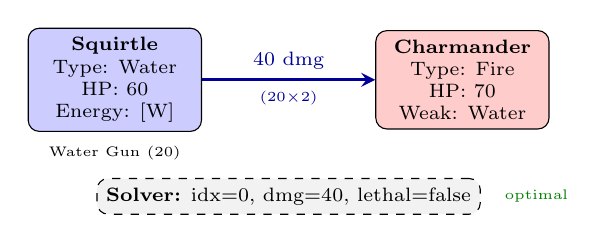
\begin{tikzpicture}[
    pokemon/.style={draw, rounded corners, minimum width=2.2cm, minimum height=1.2cm, align=center, font=\scriptsize},
    arrow/.style={->, thick, >=stealth},
    result/.style={draw, dashed, rounded corners, fill=gray!10, align=center, font=\scriptsize}
]
\node[pokemon, fill=blue!20] (squirtle) {\textbf{Squirtle}\\Type: Water\\HP: 60\\Energy: [W]};
\node[below=0.05cm of squirtle, font=\tiny] {Water Gun (20)};
\node[pokemon, fill=red!20, right=2.2cm of squirtle] (charmander) {\textbf{Charmander}\\Type: Fire\\HP: 70\\Weak: Water};
\draw[arrow, blue!60!black, very thick] (squirtle.east) -- node[above, font=\scriptsize] {40 dmg} node[below, font=\tiny] {(20$\times$2)} (charmander.west);
\node[result, below=0.6cm of $(squirtle.south east)!0.5!(charmander.south west)$] (result) {\textbf{Solver:} idx=0, dmg=40, lethal=false};
\node[right=0.1cm of result, font=\tiny, text=green!50!black] {$\checkmark$ optimal};
\end{tikzpicture}
\caption{Case study: certified solver selects Water Gun, applying $\times 2$ weakness.}
\label{fig:casestudy}
\end{figure}

\begin{lstlisting}[basicstyle=\ttfamily\small,columns=flexible]
#eval solve squirtleInPlay charmanderInPlay
-- some { attackIndex := 0, expectedDamage := 40, 
--        isLethal := false }
\end{lstlisting}

The solver correctly applies the $\times 2$ weakness multiplier ($20 \times 2 = 40$).
The soundness theorem guarantees this attack is legal; the optimality theorem guarantees no available attack deals more damage.

%%%%%%%%%%%%%%%%%%%%%%%%%%%%%%%%%%%%%%%%%%%%%%%%%%%%%%%%%%%%%%%%%%%%%%%%%%%%%%%
\section{Related Work and Future Directions}
\label{sec:related}
%%%%%%%%%%%%%%%%%%%%%%%%%%%%%%%%%%%%%%%%%%%%%%%%%%%%%%%%%%%%%%%%%%%%%%%%%%%%%%%

\paragraph{Operational Semantics and Verification.}
Our small-step semantics follows Plotkin's structural approach~\cite{Plotkin2004}.
Large-scale verification projects like CompCert~\cite{Leroy2009} and CakeML~\cite{DBLP:journals/jar/KumarHMN16} demonstrate that realistic systems can be formally verified with similar methodology.

\paragraph{Formal Game Verification.}
Prior work has formalized combinatorial games in Lean~\cite{LeanGames2022} and mechanized game-theoretic reasoning~\cite{Kerber2016}, but to our knowledge, no prior formalization addresses commercial TCG rule complexity.

\paragraph{Lean 4 Ecosystem.}
Mathlib~\cite{mathlib2020} provides mathematical foundations, while recent Lean~4 metaprogramming~\cite{Ullrich2022} enables proof automation.
Our work extends Lean~4's application domains to game rule systems.

\paragraph{Future Work.}
Directions include: stadium cards, probabilistic coin-flip reasoning, deck validation (60-card, 4-copy rule), and minimax strategy synthesis.

\paragraph{Artifact.}
The complete formalization (approximately 3{,}500 lines of Lean~4) is available at the anonymous repository.\footnote{\url{https://anonymous.4open.science/r/AnonymousLeanPokemon-8E76}}
All theorems compile without \texttt{sorry} axioms under Lean 4.26.0 with Mathlib.
\cref{tab:theorems} summarizes the key proven results.

\begin{table}[t]
\centering
\caption{Summary of key theorems proven in the formalization.}
\label{tab:theorems}
\small
\begin{tabular}{lll}
\hline
\textbf{Theorem} & \textbf{Category} & \textbf{Property} \\
\hline
\texttt{step\_total\_for\_legal} & Semantics & Legal actions always succeed \\
\texttt{step\_error\_iff\_not\_legal} & Semantics & Errors iff illegal \\
\texttt{reachable\_card\_conservation} & Invariant & Card count preserved \\
\texttt{reachable\_bench\_bounds} & Invariant & Bench $\leq 5$ \\
\texttt{no\_turn\_one\_win} & Invariant & No T1 victory possible \\
\texttt{bestAttack\_sound} & Solver & Returns legal attack \\
\texttt{bestAttack\_optimal} & Solver & Maximizes damage \\
\texttt{solveTwoPly\_optimal} & Solver & 2-turn optimality \\
\hline
\end{tabular}
\end{table}

%%%%%%%%%%%%%%%%%%%%%%%%%%%%%%%%%%%%%%%%%%%%%%%%%%%%%%%%%%%%%%%%%%%%%%%%%%%%%%%
% Bibliography
%%%%%%%%%%%%%%%%%%%%%%%%%%%%%%%%%%%%%%%%%%%%%%%%%%%%%%%%%%%%%%%%%%%%%%%%%%%%%%%

\bibliography{references}

\end{document}
